% Archetype F1 : frise a double registre (histoire humaine / phylogenie du pathogene)
\documentclass[border=4pt,varwidth=false]{standalone}
\usepackage[T1]{fontenc}
\usepackage{lmodern}
\usepackage{xcolor}
\usepackage{tikz}
\usetikzlibrary{positioning,arrows.meta,calc,fit,backgrounds}

% Palette sobre, compatible daltonisme (Okabe-Ito reduit)
\definecolor{humanblue}{HTML}{0072B2}
\definecolor{pathorange}{HTML}{D55E00}
\definecolor{neutralgrey}{HTML}{4D4D4D}
\definecolor{bandtint}{HTML}{F4F4F4}

% Echelle du temps : annee (negative = avant l'ere commune) -> centimetres.
% Deux segments d'echelles differentes separes par une rupture d'axe EXPLICITE :
% le passe profond est comprime, les derniers siecles sont dilates. Sans rupture
% visible, une echelle non lineaire est une faute de lecture, pas une commodite.
% Regle : \tx doit rester une expression evaluable par pgfmath (pas de \def a chiffres).
\newcommand{\txdeep}[1]{{(#1 + 10000)/1400}}      % -10000 .. -500  -> 0 .. 6.8
\newcommand{\txrecent}[1]{{7.6 + (#1 + 500)/280}} % -500 .. 2000    -> 7.6 .. 16.5
\newcommand{\marginleft}{-1.45}

\begin{document}
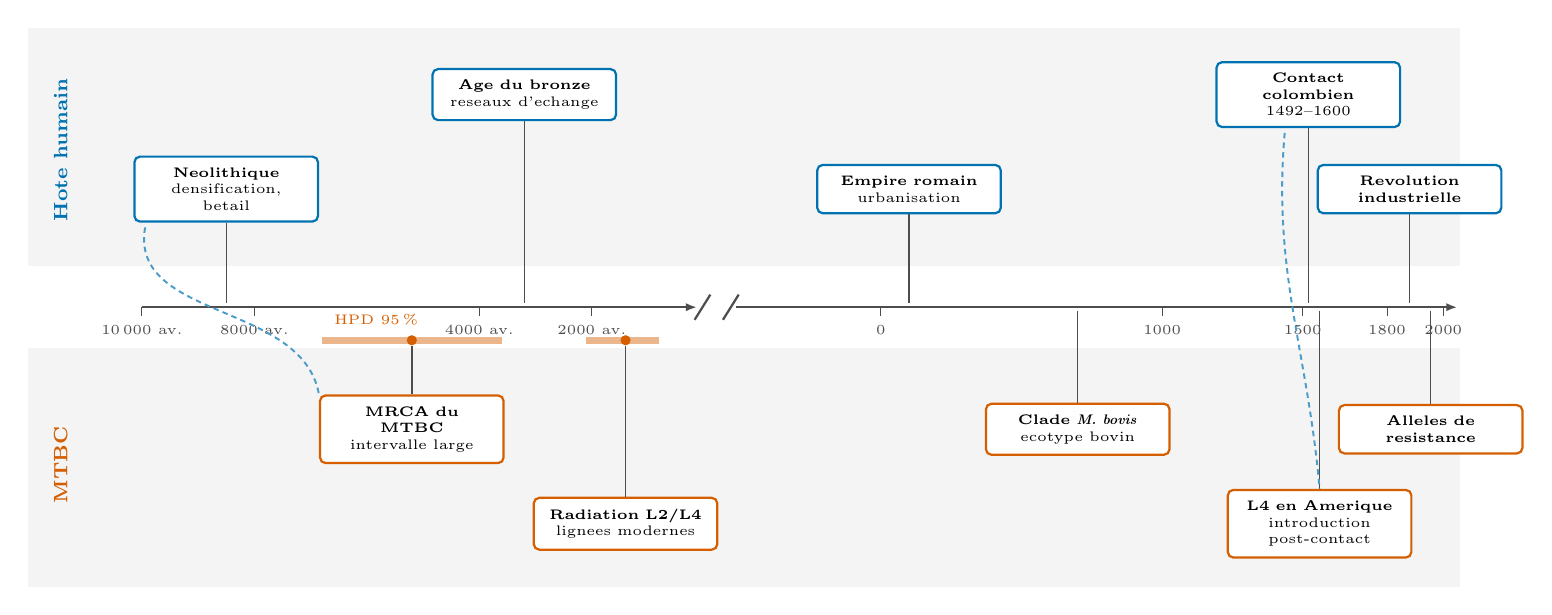
\begin{tikzpicture}[
    every node/.style={font=\scriptsize, align=center},
    evt/.style={
      draw, thick, rounded corners=2pt, inner sep=4pt,
      text width=2.05cm, font=\tiny, fill=white
    },
    human/.style={evt, draw=humanblue},
    patho/.style={evt, draw=pathorange},
    stem/.style={neutralgrey, line width=0.5pt},
    link/.style={dash pattern=on 2pt off 1.5pt, humanblue!70, line width=0.7pt},
    hpd/.style={pathorange, line width=2.4pt, opacity=0.45},
    tip/.style={circle, fill=pathorange, inner sep=1.3pt},
    axis/.style={-{Latex[length=4pt]}, neutralgrey, line width=0.8pt}
  ]

  % --- bandes de fond : un registre = une bande ---------------------------
  \begin{scope}[on background layer]
    \fill[bandtint] (\marginleft, 0.52) rectangle (\txrecent{2060}, 3.55);
    \fill[bandtint] (\marginleft, -3.55) rectangle (\txrecent{2060}, -0.52);
  \end{scope}

  % --- etiquettes de registre, dans une marge qui leur est reservee -------
  \node[font=\scriptsize\bfseries, text=humanblue, rotate=90] at (\marginleft+0.42, 2.0) {Hote humain};
  \node[font=\scriptsize\bfseries, text=pathorange, rotate=90] at (\marginleft+0.42, -2.0) {MTBC};

  % --- axe du temps et rupture d'echelle ---------------------------------
  \draw[axis] (\txdeep{-10000}, 0) -- (7.05, 0);
  \draw[axis] (7.55, 0) -- (\txrecent{2050}, 0);
  \draw[neutralgrey, line width=0.8pt] (7.02,-0.16) -- (7.22,0.16);
  \draw[neutralgrey, line width=0.8pt] (7.38,-0.16) -- (7.58,0.16);

  \foreach \yr/\lab in {-10000/{10\,000 av.}, -8000/{8000 av.}, -4000/{4000 av.}, -2000/{2000 av.}}
    {\draw[neutralgrey] (\txdeep{\yr}, 0) -- ++(0,-0.11) node[below=0pt, font=\tiny, text=neutralgrey] {\lab};}
  \foreach \yr/\lab in {0/{0}, 1000/{1000}, 1500/{1500}, 1800/{1800}, 2000/{2000}}
    {\draw[neutralgrey] (\txrecent{\yr}, 0) -- ++(0,-0.11) node[below=0pt, font=\tiny, text=neutralgrey] {\lab};}

  % --- registre superieur : evenements humains ---------------------------
  \node[human] (neo)  at (\txdeep{-8500},  1.50) {\textbf{Neolithique}\\densification, betail};
  \node[human] (bro)  at (\txdeep{-3200},  2.70) {\textbf{Age du bronze}\\reseaux d'echange};
  \node[human] (rom)  at (\txrecent{100},  1.50) {\textbf{Empire romain}\\urbanisation};
  \node[human] (col)  at (\txrecent{1520}, 2.70) {\textbf{Contact colombien}\\1492--1600};
  \node[human] (ind)  at (\txrecent{1880}, 1.50) {\textbf{Revolution\\industrielle}};
  \foreach \n in {neo,bro,rom,col,ind} {\draw[stem] (\n.south) -- (\n.south |- 0,0.05);}

  % --- registre inferieur : evenements du pathogene ----------------------
  % Une date de datation moleculaire SANS son intervalle de credibilite est une
  % affirmation non falsifiable : le HPD se dessine, il ne se relegue pas en note.
  \draw[hpd] (\txdeep{-6800}, -0.42) -- (\txdeep{-3600}, -0.42);
  \node[tip] (mrcatip) at (\txdeep{-5200}, -0.42) {};
  \draw[hpd] (\txdeep{-2100}, -0.42) -- (\txdeep{-800}, -0.42);
  \node[tip] (ltip) at (\txdeep{-1400}, -0.42) {};
  \node[font=\tiny, text=pathorange, anchor=south west] at (\txdeep{-6750}, -0.36) {HPD 95\,\%};

  \node[patho] (mrca) at (\txdeep{-5200}, -1.55) {\textbf{MRCA du MTBC}\\intervalle large};
  \node[patho] (rad)  at (\txdeep{-1400}, -2.75) {\textbf{Radiation L2/L4}\\lignees modernes};
  \node[patho] (bov)  at (\txrecent{700},  -1.55) {\textbf{Clade \emph{M. bovis}}\\ecotype bovin};
  \node[patho] (amer) at (\txrecent{1560}, -2.75) {\textbf{L4 en Amerique}\\introduction post-contact};
  \node[patho] (res)  at (\txrecent{1955}, -1.55) {\textbf{Alleles de\\resistance}};

  \draw[stem] (mrca.north) -- (mrcatip.south);
  \draw[stem] (rad.north)  -- (ltip.south);
  \foreach \n in {bov,amer,res} {\draw[stem] (\n.north) -- (\n.north |- 0,-0.05);}

  % --- connecteurs : la ou l'argument de co-evolution se joue -------------
  % Un connecteur est une HYPOTHESE TESTEE, pas une decoration : il ne relie que
  % les paires dont le recouvrement est mesure quelque part dans l'article.
  \draw[link] (neo.south west) ++(0.15,-0.06) to[out=-100,in=100] (mrca.north west);
  \draw[link] (col.south) ++(-0.3,-0.06) to[out=-95,in=95] (amer.north);

\end{tikzpicture}
\end{document}
